\documentclass{beamer}
\usepackage[utf8]{inputenc}
\usetheme{Warsaw}
\usecolortheme{crane}
\usecolortheme{orchid}
\usepackage{listings}
\usepackage{color}
\usepackage{graphicx}

\definecolor{amber}{rgb}{1.0, 0.75, 0.0}
\definecolor{darkWhite}{rgb}{0.94,0.94,0.94}
\newcommand{\TextSoulign}[3]{\emph{\textcolor{#1}{\underline{#2\textcolor{black}{#3}}}}}

\lstset{
   backgroundcolor={darkWhite}
}


\title{Package Coberny}
\author{A.Bernard, F.Chery, O.Côme}\institute{Faculté des sciences de Montpellier}
\date{13 Décembre 2021}

\begin{document}

\begin{frame}
\titlepage
\end{frame}

\begin{frame}
  \frametitle{Sommaire}
  \tableofcontents
\end{frame}

\section{Introduction}
\subsection{Création de la base de données}

\begin{frame}[fragile]{Création de la base de données}
\TextSoulign{amber}{Dataframe intermédiaire} : \newline
\begin{itemize}
\item Pour créer le data nous avons utilisé $\textbf{pandas}$ pour sélectionner uniquement les sorties d'autoroute concernées par le projet et enlever les portions gratuites.  
\item Nous avons utilisé $\textbf{pyproj}$ pour transformer les coordonnées L93 en WGS84. Nous avons donc obtenu à la suite un dataframe avec les noms des autoroutes, les noms des péages et les coordonnées GPS.
\end{itemize}
\end{frame}


\begin{frame}[fragile]{Création de la base de données}
\begin{block}{Dataframe des prix}
Nous avons simplement reporté le fichier que nous avions en format $\textit{.csv}$ pour l'utiliser avec $\textbf{pandas}$ et choisir les péages voulus. Puis nous avons renommé les colonnes pour être cohérent avec les autres dataframe.
\end{block}
\begin{block}{Dataframe des distances}
Nous avons utilisé $\textbf{requests}$ et $\textbf{json}$ pour faire des requêtes de distance entre chaque coordonnées du dataframe créé précédemment. Ces packages utilisent les données de $\textbf{openstreetmap}$.
\end{block}
\end{frame}



\subsection{Présentation du package Coberny}

\begin{frame}[fragile]{Présentation du package Coberny}
\begin{block}{Installer Coberny}
pip install git+https://github.com/ABernard27/PROJET-groupe-3
\end{block}
Ce package permet de réaliser 3 actions primaires : \newline
\begin{itemize}
\item Réaliser une carte intéractive d'un trajet sur l'autoroute en affichant les noms des stations, le prix entre deux stations et le temps en kilomètres.
\item Afficher la distribution des prix entre deux sorties
\item Déterminer, en fonction du nombre de sorties acceptées, le trajet le moins coûteux
\end{itemize}
\end{frame}



\section{Carte intéractive}
\subsection{Création de la carte}

\begin{frame}[fragile]{Création de la carte}

La carte repose sur 3 packages essentiels : $\textbf{openrouteservice}$, $\textbf{json}$ et $\textbf{folium}$. Il y a une petite manipulation en plus pour exécuter cette fonction : créer une clé API sur $\textit{openrouteservice.org}$. Le code créé exécute des requêtes avec les points de coordonnées entrés pour relier tous ses points. L'API de direction renvoie des polylignes codés (série de coordonnées sous la forme d'une seule chaîne), à l'aide de 
$\textit{convert.decode\_polyline}$ on peut les décoder. Ensuite $\textit{folium.GeoJson(decoded).add\_to(m)}$ ajoute à la carte les points reliés. $\textit{summary}$ permet de récupérer les distances dans le fichier json pour les afficher. Enfin, $\textit{folium.Marker}$ permet d'ajouter les marqueurs.
\end{frame}

\subsection{Utilisation}
\begin{frame}[fragile]{Utilisation}
Pour utiliser cette fonction les dataframe doivent être de la forme suivante : (extrait des tableaux)
\begin{center}
\begin{tabular}{|*{4}{c|}}
\hline
&MONTPELLIER&SETE&AGDE \\
\hline
0&0.0&1.6&3.6\\
\hline
1&1.6&0.0&1.9 \\
\hline
2&3.6&1.9&0.0\\
\hline
\end{tabular} \newline
Extrait tableau des prix
\end{center}
\begin{center}
\begin{tabular}{|*{4}{c|}}
\hline
&MONTPELLIER&SETE&AGDE \\
\hline
MONTPELLIER&0.0&17.0&41.0\\
\hline
SETE&17.0&0.0&26.0 \\
\hline
AGDE&41.0&26.0&0.0\\
\hline
\end{tabular} \newline
Extrait tableau des distances
\end{center}
\end{frame}

\subsection{Exemple}
\begin{frame}[fragile]{Exemple}
Par exemple pour utiliser la fonction carte il suffit d'importer $\textbf{Coberny}$ puis de taper la commande suivante : 
\begin{block}{Exemple d'utilisation}
Coberny.carte(np.column$\_$stack([data['x'],data['y']]), data[' Nom gare' ], 'Key', prix)
\end{block}
Ici data est un dataframe contenant les noms des péages ainsi que leur coordonnée (longitude, latitude), Key est la clé openrouteservice, et prix est le dataframe contenant les prix entre toutes les sections.
Après avoir exécuter ce code nous obtenons la carte suivante où l'on peut cliquer sur les marqueurs et les portions de route : 
\end{frame}

\begin{frame}[fragile]{Exemple}
\begin{center}
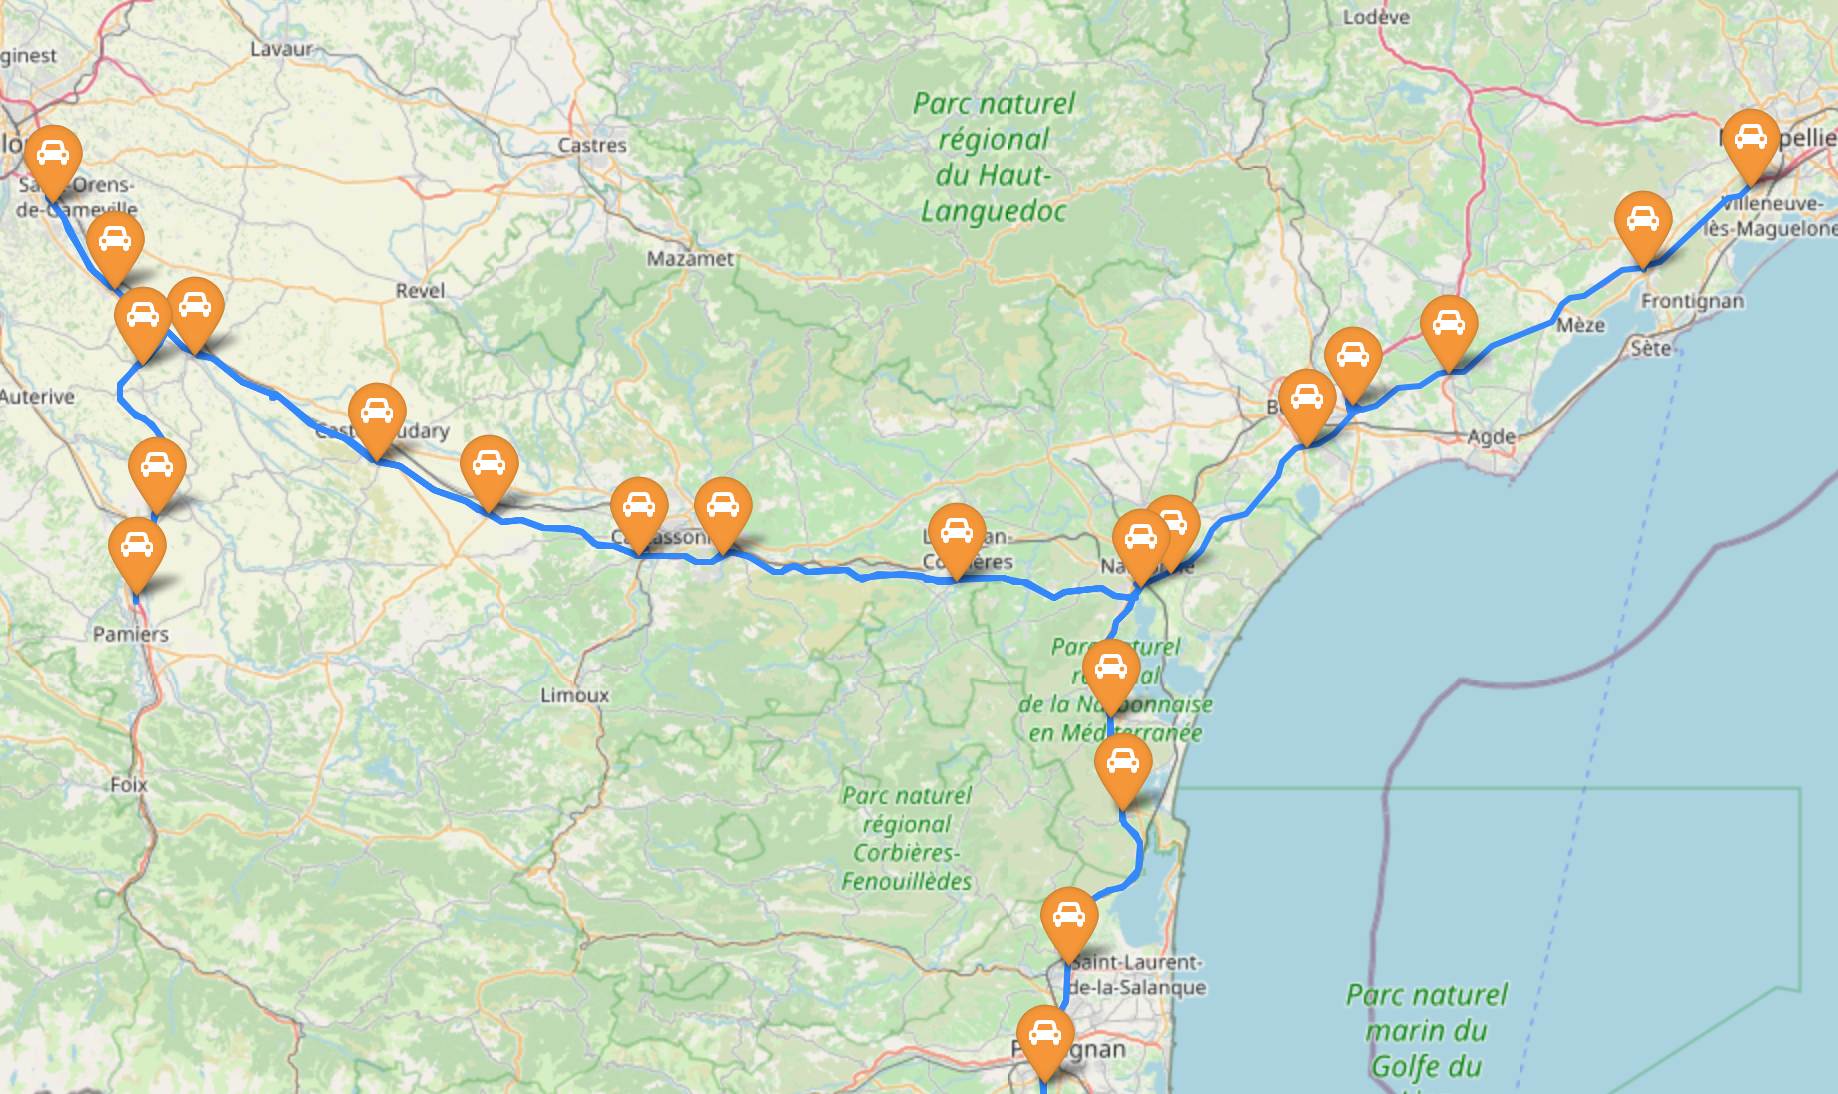
\includegraphics[scale=0.3]{carte.png}
\end{center}
\end{frame}



\section{Distribution des prix}
\begin{frame}
nzkldnz
\end{frame}

\section{Minimisation coût du trajet}
\begin{frame}
zdn kzlf dz
\end{frame}



\end{document}



